\chapter{Methodology}

\section{Section header}

\section{Algorithm}

Q-learning, a model-free online off-policy algorithm, whose main strength is that it is able to compare the expected utility of the available actions without requiring a model of the environment:

\begin{equation}
        Q(s_t, a_t) \gets Q(s_t, a_t) + \alpha [r_{t+1} + \gamma \max_a Q(s_{t+1}, a) - Q(s_t, a_t)]
\end{equation}

%%%%%%%%%%%%%%%%%%%%%%%%%%%%%%%%%%%%%%%%%%%
\subsection{Data Preprocessing}

\begin{itemize}

    \item Crop.
    
    	\begin{figure}[h]
   	 \centering
   	 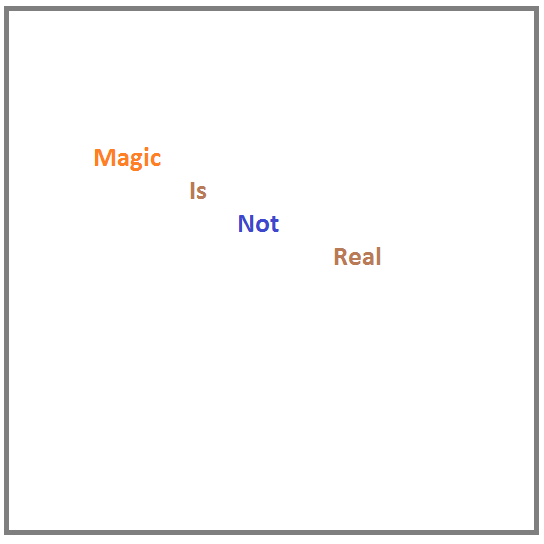
\includegraphics[width=0.5\textwidth]{figs/magic}
    	\caption{Cropped input image.}
    	\end{figure}
    
    The raw input image is captured by Universe in the function "step()" which is simply a screenshot of the browser as shown in Figure 2. Obviously the useful vision information are only from the game screen. If we go further, the top half of the game screen displaying the sky does not change very much and the bottom half of the is heavily effected by the turning actions. Thus a region of interest is carefully chosen by whether considering whether it relates to decide an expected steering behavior.  Then the image is simply cropped by a new window with the "cropFrame()" function. An example cropped image is as shown in Figure 6.   
    
    \item Downscale the resolution.

    	\begin{figure}[h]
    	\centering
   	 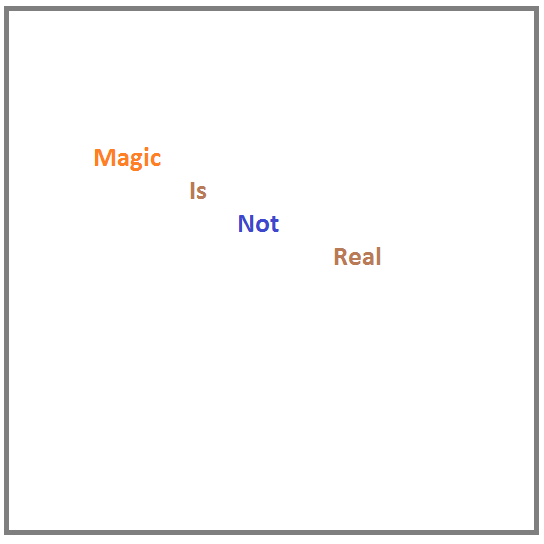
\includegraphics[width=0.25\textwidth]{figs/magic}
   	 \caption{Downsized input image.}
    	\end{figure}
    
    A high resolution is usually redundant for a computer vision task. By resizing with a smaller size, the space information are almost remained and the computing time are greatly saved. The cropped image is then downsized to a smaller size, [80, 80] as in Figure 7. Downscaling the resolution doesn't hurt the information for turning left or right but highly accelerating the computing since much smaller data are being processed.
    
    \item Grayscale.

	\begin{figure}[h]
	\centering
	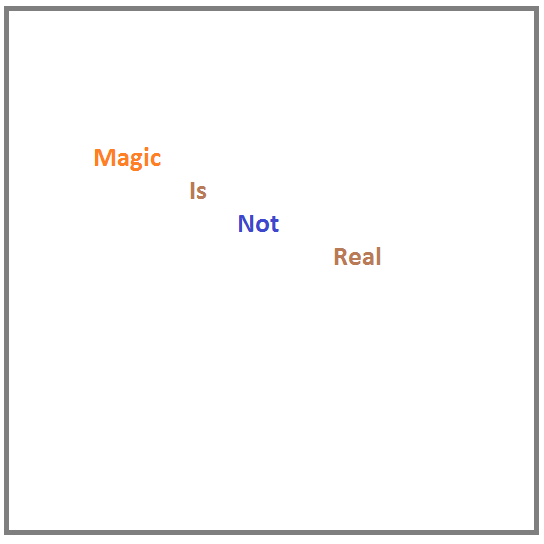
\includegraphics[width=0.25\textwidth]{figs/magic}
	\caption{Grayscaled input image.}
	\end{figure}
    
   Grayscale processing is another useful technique in computer vision tasks since it is a great help for accelerating the computing and is at least three times faster than that of color image processing. This is because grayscale image has only one color channel as opposed to three in a color image.  The color information are usually dumped when unnecessary for the computer vision tasks. As here, the downsized image is gray scaled as in Figure 8, because the color information does not help much for the steering control. 

\end{itemize}

%%%%%%%%%%%%%%%%%%%%%%%%%%%%%%%%%%%%%%%%%%%
\subsection{Implementation}

\subsubsection{Environment Setting}

OpenAI Universe is designed with using Docker so it can reset the Game continuously. Docker is a tool that lets you run virtual machines on the local computer. I created an image wrapping up everything necessary, like TensorFlow, OpenCV, Gym and Universe.

To start up a very first Game Environment, only gym and universe modules are needed. Since we are to generate some random behaviors, "random" is also imported.

...

\subsubsection{Build the Deep Neural Network}

The Deep Neural Network is based on the DeepMind paper except for the changes of input and output sizes.

...

\subsubsection{Preprocessing Functions}

As described in the previous chapters, the crop, downsample and grayscale operations are done with the following functions:

...

\subsubsection{Finetuning Hyperparameters}

I played with some hyperparameters:

\begin{itemize}
\item The number of time steps
\item The capacity of the replay memory,
\item The layers of the network and the region of interest.
\end{itemize}
Currently this process is nothing more than trial and error. I could be better designed by grid search or random search. Well, it could be even easier to design the pipeline of implement a Deep Reinforcement Learning problem but tougher in hyperparameter tuning. Without a deeper understanding of the features of model, it has a high probability to fall into a less efficient experiment process. 

%%%%%%%%%%%%%%%%%%%%%%%%%%%%%%%%%%%%%%%%%%%
\subsection{Refinement}

\subsubsection{Relay Memory}
Along the first several trials, I experimented with different memory capacities. The memory is a pool where the Game Bot would pick actions by Q values from. A small pool means it would be quick to converge during the training stage while it also limits the capacity it can learn. So there is a tradeoff here.

\subsubsection{The Complexity of the Nerwork}
The original works well for some simple game such as Atari and CartPole. The Coster Racer Game here is more complex to play because it scores by driving along the way with a high speed. The delay between an action and a reward is bigger. Through a long time training, it has a bad classification on Left Turn and Right Turn cases.

I replace the DeepMind model with LeNet-5 which then shows a better ability in classifying and quicker convergence.



%\bibliographystyle{plainnat}
%\markright{\textit{Bibliography}}
%\renewcommand{\chaptername}{}
%\bibliography{KL-Thesis}

%\end{flushleft}
%\vfill
